\documentclass[hidelinks, dutch]{article}
\usepackage{microtype}
\usepackage{babel}
\usepackage[utf8]{inputenc}
\usepackage{listings}
\usepackage[margin=1in]{geometry}
\usepackage{graphicx}
\usepackage{tikz}
\usepackage{listings}
\usepackage{amsfonts}
\usepackage{mathptmx}
\usepackage{amsmath}
\pdfmapfile{=mtpro2.map}
\usepackage[lite]{mtpro2}
\usepackage{hyperref}

\title{Mandelbrot - JavaFX}
\author{Tom Sandmann}

\date{\today}

\begin{document}
\maketitle
\lstset{language=Java}
\tableofcontents

\section{Introductie}
Hier een klein verslag van mijn poging om de mandelbrotverzameling te programmeren in javaFX. Er worden enkele belangrijke functies behandelt.

\section{Uitleg Functies}
\subsection{Tekenen van selectie}
Indien de gebruiker met de muis sleept, wordt er een rechthoek getekend die de selectie aangeeft. Als de gebruiker de muis nu loslaat wordt ingezoomd op de selectie. We moeten oppassen met het tekenen van de selectie, omdat het verschil tussen de x-waardes en y-waardes negatief kan worden. We laten eerst zien hoe de coördinaten van het scherm zijn opgebouwd:
\begin{center}
	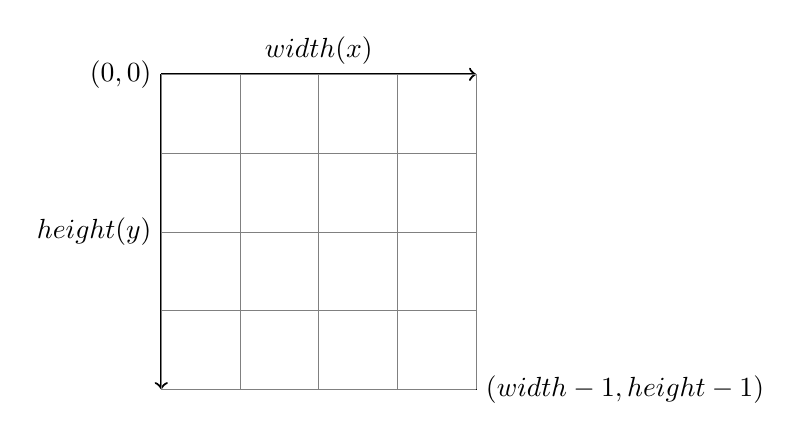
\begin{tikzpicture}
	\draw (0,0) -- (4,0) node[anchor= west] {$(width-1,height-1)$} -- (4,4) -- (0,4) node[anchor= east] {$(0,0)$} -- (0,0);
	\draw[thick,->] (0,4) -- (4,4);
	\draw[thick,->] (0,4) -- (0,0);
	\draw(0cm, 4cm) -- (2cm, 4cm) node [anchor=south] {$width(x)$};
	\draw(0cm, 4cm) -- (0cm, 2cm) node [anchor=east] {$height(y)$};
	\draw[step=1cm, gray, very thin] (0,0) grid (4,4);
	\end{tikzpicture}
\end{center}
Zoals we hierboven kunnen zien komt de $width$ overeen met het $x$ coördinaat en de $height$ met het $y$-coördinaat. Een rectangle wordt altijd getekend vanaf een bepaald coördinaat $(x,y)$ met een gespecificeerde breedte en hoogte. Als de gebruiker de muis indrukt, worden de initiële coördinaten van de muis vastgelegd als $(x_{init},y_{init})$. Tijdens het slepen (terwijl de muisknop is ingedrukt) worden nieuwe coördinaten van de muis vastgelegd als $(x_{final},y_{final})$. We hebben 4 gevallen waarbij we moeten oppassen hoe we de rechthoek tekenen. In deze gevallen is de breedte gedefinieerd als $x_{final}-x_{init}$ en de hoogte als $y_{final}-y_{init}$.

\subsubsection{Geval 1}
\begin{center}
	\begin{tikzpicture}
	\draw (0,0) -- (4,0) node[anchor= west] {$(x_{final},y_{final})$} -- (4,4) -- (0,4) node[anchor= east] {$(x_{init},y_{init})$} -- (0,0);
	\end{tikzpicture}
\end{center}
Dit is het makkelijke geval, omdat $x_{init}<x_{final}$ en $y_{init}<y_{final}$ zullen de hoogte en breedte positief zijn. We kunnen de Rechthoek gewoon maken als
\begin{lstlisting}
	Rectangle r = new  Rectangle(xInit, yInit, breedte, hoogte)
\end{lstlisting}

\subsubsection{Geval 2}
\begin{center}
	\begin{tikzpicture}
	\draw (0,0) -- (4,0) -- (4,4) node[anchor= west] {$(x_{final},y_{final})$} -- (0,4) node[anchor=east] {$(?,?)$} -- (0,0) node[anchor= east] {$(x_{init},y_{init})$};
	\end{tikzpicture}
\end{center}
We zien nu dat nog steeds $x_{init}<x_{final}$, echter is $y_{init}>y_{final}$. We moeten dus de coördinaten van $(?,?)$ berekenen. We zien dat de $x$-waarde gelijk is aan die van $x_{init}$ en dat de $y$-waarde gelijk is aan die van $y_{final}$. We krijgen dus de volgende rechthoek (let op dat de gedefinieerde hoogte nu negatief is): 
\begin{lstlisting}
Rectangle r = new  Rectangle(xInit, yFinal, breedte, abs(hoogte))
\end{lstlisting}

\subsubsection{Geval 3}
\begin{center}
	\begin{tikzpicture}
	\draw (0,0) -- (4,0) node[anchor= west] {$(x_{init},y_{init})$} -- (4,4) -- (0,4) node[anchor=east] {$(x_{final},y_{final})$} -- (0,0) ;
	\end{tikzpicture}
\end{center}
We zien nu dat de $x$- en $y$-coördinaten gelijk zijn aan die van $(x_{final},y_{final})$. omdat nu echter geldt dat $x_{final}<x_{init}$ en $y_{final}<y_{init}$ zijn zowel de gedefinieerde breedte als hoogte negatief. We krijgen dus de volgende rechthoek:
\begin{lstlisting}
Rectangle r = new  Rectangle(xFinal, yFinal, abs(breedte), abs(hoogte))
\end{lstlisting}

\subsubsection{Geval 4}
\begin{center}
	\begin{tikzpicture}
	\draw (0,0) node[anchor=east] {$(x_{final},y_{final})$} -- (4,0) -- (4,4)  node[anchor=west] {$(x_{init},y_{init})$} -- (0,4) node[anchor=east] {$(?,?)$} -- (0,0) ;
	\end{tikzpicture}
\end{center}
We moeten weer de coördinaten van $(?,?)$ berekenen. We zien dat het $x$-coördinaat gelijk  is aan $x_{final}$ en dat het $y$-coördinaat gelijk is aan $y_{init}$. Er geldt echter wel dat $x_{final}<x_{init}$ dus de gedefinieerde breedte is nu negatief. We krijgen de volgende rechthoek:
\begin{lstlisting}
Rectangle r = new  Rectangle(xFinal, yInit, abs(breedte), hoogte)
\end{lstlisting}

\subsection{Berekenen van coördinaten}
Een andere belangrijke functie is het berekenen van alle $(x,y)$ coördinaten gegeven het middelpunt met coördinaat $(a,b)$. We leggen deze functie uit d.m.v. een concreet voorbeeld. Stel we hebben het coördinaat $(1.0, 0.5)$ met een schaalfactor van $10000$ en een scherm van $500\times 500$. $\frac{1}{schaalfactor}$ geeft de stapgrootte aan langs beide assen. We hebben in dit concrete voorbeeld een stapgrootte van $\frac{1}{10000}=0.0001$. Omdat ons scherm $500\times 500$ groot is, liggen onze x coördinaten tussen $1.0-\frac{1}{2}\cdot\frac{1}{10000}=0.975$ en $1.0+\frac{1}{2}\cdot\frac{1}{10000}=1.025$. Onze y coördinaten liggen tussen $-0.5-\frac{1}{2}\cdot\frac{1}{10000}=-0.525$ en $-0.5+\frac{1}{2}\cdot\frac{1}{10000}=-0.475$. We krijgen dus de volgende algemene formule:
\begin{center}
	center = $(a,b)$, \\
	screensize = $B\times H$, \\
	scalefactor = $s$, \\
	$x \in \big[ a - \frac{1}{2} \cdot \frac{1}{s} \cdot B, a+\frac{1}{2} \cdot \frac{1}{s} \cdot B \big) $, \\
	$y \in \big[  b-\frac{1}{2} \cdot \frac{1}{s} \cdot H, b+\frac{1}{2} \cdot \frac{1}{s} \cdot H \big) $. \\
\end{center}

We krijgen de volgende functie:
\begin{lstlisting}
    public void calcCoordinates(double a, double b) {
	    double stepX = 1.0 / scalefactor;
	    double stepY = 1.0 / scalefactor;
	    double widthX = stepX * gridW;
	    double heightY = stepY * gridH;
        for (int width = 0; width < gridW; width++) {
		    for (int height = 0; height < gridH; height++) {
			    double newX = a - widthX * 0.5 + width * stepX;
			    double newY = b - heightY * 0.5 + height * stepY;
			    coordinates[width][height] = new Point(newX, newY);
		    }
	    }
    }
\end{lstlisting}
\subsubsection{Optimalisaties}
Er zijn enkele optimalisaties toe te passen voor het berekenen van de mandelwaardes voor alle coördinaten op het scherm:
\begin{itemize}
	\item Het mandelbrot figuur bestaat uit verschillende periodes. Voor punten binnen de "Main Cardioid" en "Period-2-Bulb" geldt dat de mandelwaarde altijd gelijk is aan het maximale aantal iteraties. Alvorens de coördinaten aan het Escape Time Algoritme te geven, kan dit met directe formules worden nagegaan. \\ Voor de "Main Cardioid": $p=\sqrt{(x-\frac{1}{4})^2+y^2}, x<p-2p^2+\frac{1}{4}$ \\
	Voor de "Period-2-Bulb": $(x+1)^2+y^2<\frac{1}{16}$
	
	\item Omdat de berekening van de mandelwaarde van een coördinaat los staat van andere coördinaten, kunnen we deze berekeningen verdelen. We splitsen het scherm op in blokken en laten threads voor elk van de blokken de mandelwaardes bepalen. Door de blokken niet al te groot te kiezen, versnelt dit het proces. Dit kan gerealiseerd worden door middel van een gedeelde datastructuur. Deze bevat een queue van taken die nog moeten worden uitgevoerd, en een readyqueue van taken die al zijn volbracht. Met behulp van synchronisatie moet de toegang tot deze datastructuur worden gerealiseerd. 
\end{itemize}

\subsection{Kleuringen}
De kleuring van een coördinaat hangt af van de waarde van het mandelgetal. Om een zo'n mooi mogelijk resultaat te krijgen, moeten de kleurfunctie continu zijn. Dit houdt in dat, inputwaardes die dicht bij elkaar liggen, resulteren in outputwaardes die ook dicht bij elkaar liggen. 
\subsubsection{Bernstein Polynomials}
We kunnen gebruik maken van Bernstein Polynomials, die deze eigenschap hebben. Met wat enkele aanpassingen krijgen we de volgende functies die van een gegeven mandelwaarde de kleurencodes van rood, groen en blauw bepalen (deze volgorde is willekeurig gekozen):
\begin{itemize}
	\item $t=\frac{\texttt{mandelwaarde}}{\texttt{max iterations}}$
	\item $r(t)=9\cdot (1-t)\cdot t^3$
	\item $g(t)=15\cdot (1-t)^2\cdot t^2$
	\item $b(t)=8.5\cdot (1-t)^3\cdot t$
\end{itemize}
Een plot van deze functies:
\begin{center}
		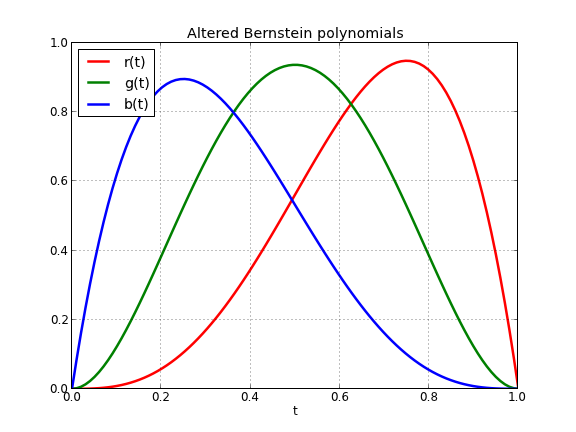
\includegraphics[scale=0.3]{img/rgb_smooth}
\end{center}
Zoals te zien is leveren deze functies allemaal een resultaat op dat ligt tussen de $0$ en de $1$. Door deze waardes met $255$ te vermenigvuldigen krijgen en te casten naar \texttt{int} krijgen we de juiste kleurenindex.

\subsubsection{Normalized Iteration Count}
Een andere manier is Normalized Iteration Count. De formule luidt als volgt: $v(z)=n-\log_P(\frac{\log|z_n|}{\log(N)})$.\\
$v(z)$ is hier een reëel getal, $n$ is het aantal iteraties, $z=x\cdot x+y\cdot y$, $P=2.0$ en $N=2.0$. Dit levert een getal op tussen $0$ en $1$. We hebben nu een cyclische rij van kleuren nodig, waaruit we een kleur gaan kiezen. Hier gaan we echter niet verder op in.

\section{Conclusie}
In het begin ondervond ik wat moeilijkheden met het kleuren van het scherm. Dit kwam omdat de x en y coördinaten van een pixel op het scherm een andere positie aangeven dan dezelfde coördinaten in het assenstelsel dat wij gewend zijn in de wiskunde. Het leuke van dit project is, dat er verschillende aspecten van het programmeren aan bod komen: GUI, multithreading, recursie en user input (d.m.v. de muis). Ik ben ook zeer tevreden met het resultaat. Er zijn nog een paar dingen die ik in de toekomst toe zou willen voegen:
\begin{itemize}
	\item gebruiker kan coördinaten intypen in een verschillende velden en aangeven dat er ingezoomd moet worden
	\item deze velden geven altijd de meest recente coördinaten aan
	\item als er ingezoomd wordt, geeft een laadbalk aan hoever de berekening is voordat het scherm de nieuwe
	resultaten laat zien.
	\item gebruiker kan uit een kleuren palette verschillende punten kiezen die de basis voor de kleuring vormen. Deze gekozen kleuring wordt vervolgens toegepast.
\end{itemize}
\end{document}
